\documentclass[a4paper,12pt]{article}
\usepackage[left=1cm,right=1cm,top=3cm,bottom=3cm,a4paper]{geometry}
\usepackage{amsmath}
\usepackage[pdftex]{graphicx}
\usepackage{graphicx}
\usepackage{kotex}
\usepackage[onehalfspacing]{setspace}
\begin{document}
	\begin{flushleft}
	고전역학 (Lagrange multiplier, Lagrangian mechanics) 리뷰
	\end{flushleft}
\paragraph{Lagrange multiplier}
라그랑지 곱수법은 어떤 constraint $\phi(x,y)=const.$가 주어져 있을 때 함수 $f(x,y)$의 최대,최솟값을 간단하게 구할 수 있는 방법이다.
\begin{flushleft}
	먼저, $f(x,y)$의 최대/최소 점을 찾고 싶으므로 $df=0$으로 둔다.( $\phi(x,y)=const.$는 당연히 $d\phi=0$ 이다.)
	$$df=\frac{\partial f}{\partial x}dx+\frac{\partial f}{\partial y}dy=0$$
	$$d\phi=\frac{\partial \phi}{\partial x}dx+\frac{\partial \phi}{\partial y}dy=0$$
\end{flushleft}
\begin{flushleft}
	그 다음, $d\phi$에 lagrange multiplier $\lambda$를 곱하고 $df$에 더한다. (이제 우리가 할 일은 $\lambda$를 찾아서 알맞은 $x,y$값을 구하는 것이다.)
	$$\left(\frac{\partial f}{\partial x}+\lambda \frac{\partial \phi}{\partial x}\right)dx+\left(\frac{\partial f}{\partial y}+\lambda \frac{\partial \phi}{\partial y}\right)dy=0 $$
\end{flushleft}
\begin{flushleft}
	이제 우리에게는 다음 세 개의 식과 세 개의 미지수($x,y,\lambda$)가 남았다.
	$$\frac{\partial f}{\partial x}+\lambda \frac{\partial \phi}{\partial x}=0,\quad\frac{\partial f}{\partial x}+\lambda \frac{\partial \phi}{\partial x}=0,\quad \phi(x,y)=0$$
\end{flushleft}
\begin{flushleft}
	앞의 두 식은 constraint $\phi(x,y)$와 함수 $f(x,y)$로 이루어진 함수 $F(x,y)=f(x,y)+\lambda\phi(x,y)$의 두 편미분이다.  
\end{flushleft}
\fbox{\begin{minipage}{30em}
		Example. 모서리가 각 축에 평행하고 타원체
	$$\frac{x^2}{a^2}+\frac{y^2}{b^2}+\frac{z^2}{c^2}=1$$
	안에 접하는 직육면체의 최대 부피를 구하여라.(Boas p.224) 
\end{minipage}}
	\begin{figure}[h]
		\centering
		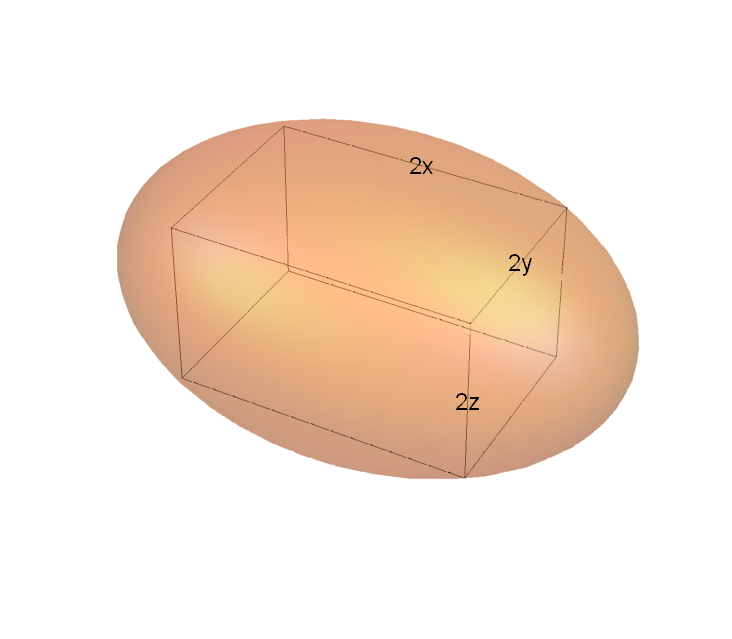
\includegraphics[width=0.3\columnwidth]{fig1.png}
		\caption{타원체에 접하는 상자}
	\end{figure}\\
Solution. 그림에서 볼 수 있듯이 타원체에 접하는 상자의 부피는 $f(x,y,z)=(2x)(2y)(2z)=8xyz$ 이고 constraint는 타원의 방정식이다. 따라서 $F(x,y,z)$는 다음과 같다.
$$F(x,y,z)=f(x,y,z)+\lambda\phi(x,y,z)=8xyz+\lambda\left(\frac{x^2}{a^2}+\frac{y^2}{b^2}+\frac{z^2}{c^2}\right) $$
세 개의 편미분을 구하면,
$$\partial_x F=8yz+\lambda\frac{2x}{a^2}=0$$
$$\partial_y F=8zx+\lambda\frac{2y}{a^2}=0$$
$$\partial_z F=8xy+\lambda\frac{2z}{a^2}=0$$
첫 번째 식에 $x$, 두 번째 식에 $y$, 세 번째 식에 $z$를 곱하고 더하면,
$$3(8xyz)+2\lambda\left(\frac{x^2}{a^2}+\frac{y^2}{b^2}+\frac{z^2}{c^2} \right)=0 $$
$\phi(x,y,z)=1$ 을 이용하면,
$$24xyz+2\lambda=0 ,\quad \lambda=-12xyz$$
이제 우리가 구한 $\lambda$를 $\partial_xF$에 넣어서 $x$를 구하자.
$$8yz-12xyz\frac{2x}{a^2}=0$$
양변을 $yz$로 나누면, 
$$x^2=\frac{1}{3}a^2$$
대칭성에 의해, 
$$y^2=\frac{1}{3}b^2,\quad z^2=\frac{1}{3}c^2$$
즉, $f(x,y,z)=8xyz$의 최댓값은 $8abc/{3\sqrt{3}}$ 이다.\\
\begin{flushleft}
	한편, constraint가 2개 이상일 땐 $F(q_1,q_2,\cdots)$을 다음과 같이 두면 된다. 
	$$F(q_1,q_2,\cdots)=f(q_1,q_2,\cdots)+\lambda_1\phi_1+\lambda_2\phi_2+\cdots$$
\end{flushleft}

\paragraph{Lagrangian mechanics}
\begin{flushleft}
	1. 어떤 입자의 운동 에너지가 $T$, 포텐셜 에너지가 $V$일 때, 이 입자의 Lagrangian $L$은 $T-V$이다.
\end{flushleft}
\begin{flushleft}
	2. Lagrangian equation of motion for a conservative system
	$$\frac{\partial L}{\partial q_i}-\frac{d}{dt}\left(\frac{\partial L}{\partial \dot{q_i}} \right)=0 $$
\end{flushleft}
\begin{flushleft}
	3. Force of constraint $f(q_1,q_2,\cdots,t)=0$ 가 있을 때, Lagrange multiplier의 응용
	$$
	dL=\sum_{i}^{3N}\left( \frac{\partial L}{\partial q_i}-\frac{d}{dt}\frac{\partial L}{\partial \dot{q_i}}\right)dq_i=0 
	$$
	$$df=\sum_{i}^{3N}\left( \frac{\partial f}{\partial q_i}\right)dq_i=0 $$
	위에서 했던 것처럼 constraint의 variation $df$에 Lagrange multiplier $\lambda(t)$를 곱하고 $dL$과 더해준다.
	$$\sum_{i}^{3N}\left( \frac{\partial L}{\partial q_i}-\frac{d}{dt}\frac{\partial L}{\partial \dot{q_i}}+\lambda(t) \frac{\partial f}{\partial q_i}\right)dq_i=0$$
	따라서,
	$$\frac{\partial L}{\partial q_i}-\frac{d}{dt}\frac{\partial L}{\partial \dot{q_i}}+\lambda(t) \frac{\partial f}{\partial q_i}=0$$
	을 풀면 된다. 이때 
	$$Q_i=\lambda(t)\frac{\partial f}{\partial q_i}$$ 를 generalized force of constraint 라고 부른다. (e.g. $q_i$가 angular coordinate일 때 $Q_i$는 토크이다.) 
\end{flushleft}
\begin{flushleft}
	4. Generalized forces (Fowles 책 chap.10 참고!)\\
	D'Alembert's principle은 뉴턴의 운동 제 2법칙(가속도의 법칙)에 해당하는 원리이다. ``구속력 혹은 반작용 힘의 가상 변위에 대한 일은 0 이다.''(위키피디아)
	$$\sum_{i}^{3N}(F_i-\dot{p_i})dx_i=0, \quad F_i=\dot{p_i}$$
	한편, 위 식의 첫 항은 virtual work라고 부르고 두 번째 항은 inertial term이라고 한다. \\
	$$\mbox{virtual work }\rightarrow\quad dW=\sum_{i}F_idx_i=\sum_{j}\left[\sum_{i}\left( F_i\frac{\partial x_i}{\partial q_j}\right)  \right]dq_j=\sum_{j}Q_jdq_j $$
	$$\mbox{inertial term }\rightarrow\quad \sum_{i}\dot{p_i}dx_i=\sum_{j}\left[\frac{d}{dt}\left(\frac{\partial T}{\partial \dot{q_j}} \right)-\frac{\partial T}{\partial q_j}  \right]dq_j \quad \mbox{:Fowles 10.8.14식} $$
	여기서 $Q_j$를 generalized forces corresponding to the generalized coordinates $q_j$ 라고 한다. 일반화 좌표 $q_j$에 대한 일반화 된 힘으로 해석할 수 있다.
\end{flushleft}
\begin{flushleft}
	5. 어떤 입자의 운동에너지가 $T$이고, 포텐셜 에너지가 $V$일 때, 그 입자의 Hamiltonian은 $H=T+V$이다.\\
	6. 다음 Hamiltonian function을 생각하자.
	$$H=\sum_{i}\dot{q_i}p_i-L, \quad L(q_i,\dot{q_i})=T(q_i,\dot{q_i})-V(q_i)$$
	note that generalized momenta conjugate to the generalized coordinate $q_i$ is
	$$p_i=\frac{\partial L}{\partial \dot{q_i}}$$
	그러면 Lagrange's e.o.m 은
		$$\frac{\partial L}{\partial q_i}-\frac{d}{dt}\left(\frac{\partial L}{\partial \dot{q_i}} \right)=\frac{\partial L}{\partial q_i}-\frac{d}{dt}(p_i)=0 $$
		$$\implies\dot{p_i}-\frac{\partial L}{\partial q_i}=0,\quad \dot{p_i}=\frac{\partial L}{\partial q_i}$$
	Hamiltonian $H$의 variataion을 구하면,
	$$dH=\sum_{i}\left[p_id\dot{q_i}+\dot{q_i}dp_i-\frac{\partial L}{\partial \dot{q_i}}d\dot{q_i}-\frac{\partial L}{\partial q_i}dq_i \right] $$
	$$=\sum_{i}\left[p_id\dot{q_i}+\dot{q_i}dp_i-p_id\dot{q_i}-\frac{\partial L}{\partial q_i}dq_i \right]$$
	$$=\sum_{i}\left[\dot{q_i}dp_i-\dot{p_i}dq_i \right]$$
	한편 $dH(p_i,q_i)$을 아래와 같이 나타낼 수 있으므로,
	$$dH=\sum_{i}\left[\frac{\partial H}{\partial p_i}dp_i+\frac{\partial H}{\partial q_i}dq_i \right] $$
	다음이 성립한다. (Hamiltion's equation)
	$$\frac{\partial H}{\partial p_i}=\dot{q_i}$$
	$$\frac{\partial H}{\partial q_i}=-\dot{p_i}$$
\end{flushleft}

\end{document}